\documentclass[a4paper,11pt]{article}

\usepackage[T1]{fontenc}
\usepackage[utf8]{inputenc}
\usepackage[english]{babel}
\usepackage[margin=2.3cm]{geometry}
\usepackage{parskip}
\usepackage{microtype}
\usepackage{xcolor}
\usepackage{listings}
\usepackage{hyperref}
\usepackage{booktabs}
\usepackage{longtable}
\usepackage{enumitem}
\usepackage{titlesec}
\usepackage{fancyhdr}
\usepackage{tikz}
\usetikzlibrary{arrows.meta,positioning,shapes.geometric,fit,backgrounds}

\hypersetup{colorlinks=true,linkcolor=blue!55!black,urlcolor=blue!55!black}

\lstdefinestyle{cpp}{
    language=C++,
    basicstyle=\ttfamily\footnotesize,
    keywordstyle=\color{blue!70!black}\bfseries,
    commentstyle=\color{green!45!black}\itshape,
    stringstyle=\color{red!60!black},
    numbers=left, numberstyle=\tiny\color{gray}, numbersep=6pt,
    frame=single, rulecolor=\color{gray!40},
    breaklines=true, showstringspaces=false, tabsize=4,
    captionpos=b,
}
\lstset{style=cpp}

\titleformat{\section}{\Large\bfseries}{\thesection}{0.8em}{}
\titleformat{\subsection}{\large\bfseries}{\thesubsection}{0.7em}{}
\titleformat{\subsubsection}{\normalsize\bfseries}{\thesubsubsection}{0.6em}{}

\pagestyle{fancy}
\fancyhf{}
\rhead{\small MirrorRoomSimulation}
\lhead{\small Developer Documentation}
\cfoot{\thepage}

\newcommand{\file}[1]{\texttt{#1}}
\newcommand{\code}[1]{\texttt{#1}}

\title{\textbf{MirrorRoomSimulation}\\[0.3em]
       \large Developer Documentation\\[0.2em]
       \normalsize (accurate as of the current state of the code)}
\author{Repository: \texttt{Githu228i/MirrorRoomSimulation}}
\date{\today}

\begin{document}
\maketitle

\begin{abstract}
\noindent
This document is a map of the project for a programmer opening
\file{MirrorRoomSimulation} for the first time. It covers where things
live, how the architecture is organized, where the actual computational
logic sits (spoiler: \emph{not} in \file{backendoperators.cpp} — that
file is empty), how to extend the code, and what pitfalls exist. It was
written by reading the sources, not by reading the original design
intent.
\end{abstract}

\tableofcontents
\newpage

% ============================================================
\section{About the project}

\file{MirrorRoomSimulation} is an educational / demo C++ application
with a Qt~6 (Widgets) GUI. The user clicks with the mouse to build a
closed (or open) chain of mirrors inside a ``room'', edits vertices and
mirror types through dialogs, and can then trace a ray bouncing off
the mirrors.

\subsection{Tech stack}

\begin{longtable}{@{}p{4cm}p{10.5cm}@{}}
\toprule
\textbf{Component} & \textbf{Purpose} \\ \midrule
\endhead
C++17 & Language. \\
Qt~6 (Widgets) & GUI, \code{QPainter}, dialogs, signals/slots. \\
CMake $\geq$ 3.16 & Build system. \\
Qt Creator & Recommended IDE. \\
\code{clangd} & Optional, for navigation. \\
\bottomrule
\end{longtable}

\subsection{Quick start}

\begin{lstlisting}[language=bash,caption={Build}]
cmake -S . -B build/Desktop-Debug -DCMAKE_BUILD_TYPE=Debug
cmake --build build/Desktop-Debug -j
./build/Desktop-Debug/MirrorRoomSimulation
\end{lstlisting}

\begin{quote}
\textbf{Important.} \file{build/}, \file{.qtcreator/},
\file{CMakeLists.txt.user}, \file{*.back*}, \file{.cache/} must
\textbf{not} be committed to Git. See~\ref{sec:git}.
\end{quote}

% ============================================================
\section{Repository structure}

\begin{longtable}{@{}p{5.8cm}p{8.7cm}@{}}
\toprule
\textbf{File} & \textbf{Purpose} \\ \midrule
\endhead
\file{main.cpp} & \code{QApplication}, translator setup, launches \code{MainWindow}. \\
\file{mainwindow.h/.cpp} & Main window. Mouse handling, \code{paintEvent}, dialog invocation. \\
\file{mainwindow.ui} & Empty design file: just \code{centralwidget}, \code{menubar}, \code{statusbar}. All rendering is done manually in \code{paintEvent}. \\
\file{points.h/.cpp} & \code{Points} (base point) and \code{Beam} (ray: point + angle). \\
\file{mirror.h/.cpp} & \code{Mirror} class hierarchy and its subclasses. Mirror intersections. Drawing. \\
\file{polygon.h/.cpp} & \code{Polygon}: a set of mirrors, closure checks, validation, ray tracing. \\
\file{frontendoperators.h/.cpp} & Scene manager: \code{CreatePoint}, \code{ConnectPoints}, \code{ChangeMirror}. \\
\file{backendoperators.h/.cpp} & \textbf{Empty stub.} Constructor only. No logic. \\
\file{changeorconnectdialog.h/.cpp} & Dialog with two buttons: ``Edit'' / ``Connect''. \\
\file{changepointdialog.h/.cpp} & Vertex editing dialog. Defines \code{ChangePointData}. \\
\file{MirrorRoomSimulation\_ru\_RU.ts} & Translation file (empty). \\
\file{README.md} & One line. \\
\file{CMakeLists.txt} & Build. \\
\bottomrule
\end{longtable}

\begin{quote}
\textbf{Orientation tip.} If you are looking for ``where the backend
logic is'' — go to \file{polygon.cpp} (ray tracing) and
\file{mirror.cpp} (intersections). \file{backendoperators.cpp} is a
skeleton that was apparently meant to be filled in but never was.
\end{quote}

% ============================================================
\section{Architecture}

\subsection{Layers}

\begin{enumerate}[label=\textbf{\arabic*.},leftmargin=*]
    \item \textbf{Geometry primitive:} \code{Points}, \code{Beam}.
    \item \textbf{Mirror model:} \code{Mirror} and subclasses + intersection
          algorithms (inside an anonymous namespace in \file{mirror.cpp}).
    \item \textbf{Scene composition:} \code{Polygon} — holds the vector of
          mirrors, traces rays, validates the contour.
    \item \textbf{Scene manager:} \code{FrontEndOperators} — a wrapper over
          \code{Polygon} for UI operations.
    \item \textbf{GUI:} \code{MainWindow} + dialogs.
\end{enumerate}

\begin{quote}
\textbf{Rule.} The model (\code{Points}, \code{Mirror}, \code{Polygon})
must not know about \code{QMainWindow}. However, \code{Polygon} already
knows about \code{QPainter} — \code{Mirror} subclasses know how to draw
themselves. This is a deliberate simplification
(see~\ref{sec:known-issues}).
\end{quote}

\subsection{Class hierarchy}

\begin{center}
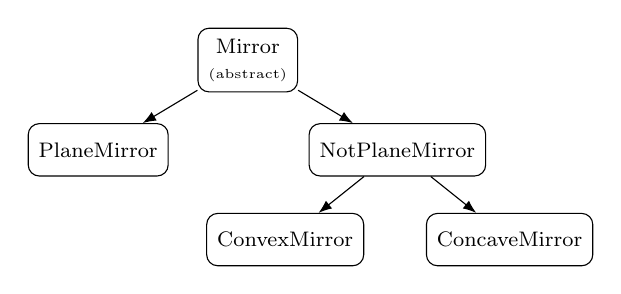
\begin{tikzpicture}[
    every node/.style={draw, rounded corners, font=\footnotesize,
                       minimum height=0.7cm, align=center, inner sep=4pt},
    edge from parent/.style={draw, -Latex},
    level 1/.style={sibling distance=4cm, level distance=1.2cm},
    level 2/.style={sibling distance=3cm, level distance=1.2cm},
    level 3/.style={sibling distance=2.5cm, level distance=1.2cm},
    scale=0.95, transform shape
]
\node (Mirror) {Mirror\\\tiny (abstract)}
    child { node (Plane) {PlaneMirror} }
    child { node (NotPlane) {NotPlaneMirror}
        child { node (Conv) {ConvexMirror} }
        child { node (Conc) {ConcaveMirror} }
    };
\end{tikzpicture}
\end{center}

\begin{itemize}[leftmargin=*]
    \item \code{Mirror} — abstract base. Fields:
          \code{start\_}, \code{end\_}, \code{rad\_}.
          Virtual destructor is mandatory — stored as
          \code{std::unique\_ptr<Mirror>}.
    \item \code{PlaneMirror} — flat mirror (rad = 0). Overrides
          \code{isFlat()} $\to$ \code{true}.
    \item \code{NotPlaneMirror} — intermediate class with a protected
          constructor.
    \item \code{ConvexMirror} — \code{rad > 0}, circle center ``left''
          of the chord.
    \item \code{ConcaveMirror} — \code{rad < 0}, center ``right''.
\end{itemize}

\subsection{Data flow}

\begin{enumerate}[leftmargin=*]
    \item User clicks in \code{MainWindow::mousePressEvent}.
    \item \code{MainWindow} decides: hit a vertex, too close, new vertex.
    \item It calls one of \code{FrontEndOperators}: \code{CreatePoint},
          \code{ConnectPoints}, or \code{ChangeMirror}.
    \item That method manipulates \code{Polygon::sides\_}
          (\code{std::vector<std::unique\_ptr<Mirror>>}).
    \item \code{MainWindow} calls \code{update()} — repaint.
    \item \code{MainWindow::paintEvent} draws \code{first} and all mirrors
          via their virtual \code{Draw()}.
\end{enumerate}

% ============================================================
\section{Key entities}

\subsection{Points and Beam (\file{points.h})}

\begin{lstlisting}[caption={Points / Beam}]
class Points {
public:
    Points(double x = 0.0, double y = 0.0);
    virtual ~Points() = default;
    double getX() const;
    double getY() const;
    double Dist(const Points& other) const;
    virtual std::string Cords() const;
protected:
    double x_, y_;
};

class Beam : public Points {
public:
    Beam(double x = 0.0, double y = 0.0, double angle = 0.0);
    double getA() const;
    std::string Cords() const override;
private:
    double angle_;
};
\end{lstlisting}

\begin{quote}
\code{Cords()} returns a string of the form \code{"x y"} (or
\code{"x y angle"} for a beam) with 3 decimal places. It is only used
for debug file output.
\end{quote}

\subsection{The Mirror hierarchy (\file{mirror.h})}

Key \code{Mirror} methods:

\begin{longtable}{@{}p{6.3cm}p{8.2cm}@{}}
\toprule
\textbf{Method} & \textbf{Purpose} \\ \midrule
\endhead
\code{Mirror(st, end, rad)} & Throws \code{std::invalid\_argument} on zero chord or $|rad| < d/2$. \\
\code{isFlat()} & \code{true} if $|rad| < 10^{-9}$ or $> 10^{7}$. \\
\code{CircleCenter()} & Circle center; side determined by the sign of \code{rad}. \\
\code{CircleCenter(bool leftSide)} & Explicit side selection. \\
\code{PointOnArc(p, c)} & Whether a point lies on the arc/segment. \\
\code{Intersections(other)} & Vector of intersection points. \\
\code{Touches(other)} & \code{!Intersections().empty()}. \\
\code{Crossing(other)} & Intersect at more than just shared endpoints. \\
\code{Draw(painter, insideOnLeft)} & Virtual. Pure virtual in the base. \\
\bottomrule
\end{longtable}

Meaning of the \code{rad\_} sign:
\begin{itemize}[leftmargin=*]
    \item $rad > 0$ — center \emph{left} of the direction
          \code{start → end}. Corresponds to \code{ConvexMirror}.
    \item $rad < 0$ — center \emph{right}. Corresponds to
          \code{ConcaveMirror}.
    \item $rad = 0$ — segment (\code{PlaneMirror}).
\end{itemize}

\subsection{Polygon (\file{polygon.h})}

The scene container.

\begin{lstlisting}[caption={Polygon fields}]
class Polygon {
    // ...
private:
    std::vector<std::unique_ptr<Mirror>> sides_;
    Points first;             // first point of an open contour
    bool isExist_ = false;    // whether the first point exists
    bool isCycled_ = false;   // whether the contour is closed
    Beam beam_;               // beam for tracing
};
\end{lstlisting}

Key methods:

\begin{longtable}{@{}p{5.5cm}p{9cm}@{}}
\toprule
\textbf{Method} & \textbf{What it does} \\ \midrule
\endhead
\code{Push(const Mirror\&)} & Copies the mirror via \code{dynamic\_cast} and appends to \code{sides\_}. Calls \code{Write()}. \\
\code{Del(int idx)} & Removes a mirror by index. Calls \code{Write()}. \\
\code{Check()} & Validation: contour is closed, sides intersect only at shared vertices of neighbors. \\
\code{TraceBeam(maxBounces)} & Ray tracing. Writes \file{beam.txt}. \\
\code{Write()} & Dumps vertices and beam to \file{points.txt}. \\
\bottomrule
\end{longtable}

\begin{quote}
\textbf{Side effect.} \code{Push}, \code{Del}, \code{Write},
\code{TraceBeam} open files. Under heavy editing this can slow things
down and clutter the working directory.
\end{quote}

\subsection{FrontEndOperators (\file{frontendoperators.h})}

\begin{lstlisting}[caption={FrontEndOperators}]
class FrontEndOperators {
public:
    FrontEndOperators();
    void CreatePoint(double x, double y);
    void ConnectPoints(int num);
    void ChangeMirror(int num, const ChangePointData &data);
    friend class MainWindow;
private:
    Polygon prototype;
};
\end{lstlisting}

\begin{quote}
\textbf{Misleading name.} This is a \emph{scene manager}, not a
rendering layer. Rendering lives in \code{MainWindow::paintEvent} and
\code{Mirror::Draw}.
\end{quote}

Method logic:
\begin{itemize}[leftmargin=*]
    \item \code{CreatePoint} — adds a new point. If \code{isExist\_} is
          false, stores \code{first} and sets the flag. Otherwise,
          builds a \code{PlaneMirror} from the end of the last mirror
          to the new point. Limit: 8 points
          (\code{if (prototype.sides\_.size() < 8)}).
    \item \code{ConnectPoints(num)} — closes the contour: erases the
          mirrors before \code{num}, adds a final mirror from
          \code{end} to \code{start}, sets \code{isCycled\_ = true}.
    \item \code{ChangeMirror(num, data)} — the most complex function.
          Handles cases: last point of an open contour, first point of
          a closed one, regular point. Everywhere it uses
          \code{dynamic\_cast} to determine the mirror type and
          recreates adjacent mirrors.
\end{itemize}

\subsection{MainWindow (\file{mainwindow.h})}

Only two fields:
\begin{lstlisting}
Ui::MainWindow *ui;
FrontEndOperators polygonCreator;
\end{lstlisting}

Logic:
\begin{itemize}[leftmargin=*]
    \item \code{mousePressEvent} — all click handling. Hardcoded:
          \code{y > 1000} is ignored, hit radius \code{25}, minimum
          distance between points \code{100}.
    \item \code{paintEvent} — draws \code{first}, the line from
          \code{first} to \code{temp[0]->getStart()}, and all mirrors.
\end{itemize}

\subsection{Dialogs}

\code{ChangeOrConnectDialog} — simple two-button window
(\code{accept} / \code{reject}). Placeholder text:
\code{"ТУТ БУДЕТ ТВОЙ ТЕКСТ"} (``your text goes here'').

\code{ChangePointDialog} — single-vertex editing. Returns:

\begin{lstlisting}
struct ChangePointData {
    double x;
    double y;
    int mirrorType;   // 0 = plane, 1 = concave, 2 = convex
    double radius;
};
\end{lstlisting}

If \code{lastPoint == true}, the mirror-type combo box and the radius
field are disabled (the last vertex has no mirror yet).

\subsection{BackEndOperators — an empty stub}

\begin{lstlisting}[caption={The entire backendoperators.cpp}]
#include "backendoperators.h"
BackEndOperators::BackEndOperators() {}
\end{lstlisting}

\begin{quote}
\textbf{Important.} Do not look for logic here. There is none. All
computational code lives in \file{mirror.cpp} and \file{polygon.cpp}
inside unnamed \code{namespace \{ \}} blocks. If you want to add
something ``to the backend'', either fill in \code{BackEndOperators}
or create a new module — do not keep spreading logic across
\file{polygon.cpp}.
\end{quote}

% ============================================================
\section{User interaction}

\subsection{Creating a point}

Click on empty space:
\begin{enumerate}[leftmargin=*]
    \item If you hit an existing point ($\le 25$) — edit it.
    \item If too close to an existing point ($\le 100$) — message ``Точки слишком близко!'' (``Points too close!'').
    \item Otherwise — \code{CreatePoint(x, y)}.
\end{enumerate}

Limit: \textbf{8 sides}.

\subsection{Editing a point}

Click on an existing point:
\begin{itemize}[leftmargin=*]
    \item \textbf{Contour closed} — \code{ChangePointDialog} opens
          directly.
    \item \textbf{Contour open} — \code{ChangeOrConnectDialog} opens
          first (``Edit'' or ``Connect'').
\end{itemize}

\subsection{Connecting points}

Choosing ``Connect'' in an open contour:
\begin{itemize}[leftmargin=*]
    \item The last mirror cannot be connected —
          \code{QMessageBox::critical}.
    \item Otherwise \code{ConnectPoints(i)}: erases all mirrors before
          \code{i}, adds one closing mirror.
\end{itemize}

% ============================================================
\section{Geometric algorithms}

\subsection{Intersections (\file{mirror.cpp}, anonymous namespace)}

\begin{itemize}[leftmargin=*]
    \item \code{IntersectSegments} — segment/segment, including the
          collinear case with overlap computation.
    \item \code{IntersectSegmentArc} — segment/arc, quadratic equation.
    \item \code{IntersectArcs} — arc/arc, standard two-circle
          intersection with \code{PointOnArc} verification.
\end{itemize}

Constants:
\code{EPS = 1e-9}, \code{POINT\_EPS = 1e-6}, \code{PAR\_EPS = 1e-10},
\code{FLAT\_R = 1e7}.

\subsection{Ray tracing (\file{polygon.cpp})}

\code{TraceBeam}:
\begin{enumerate}[leftmargin=*]
    \item Position and direction come from \code{beam\_}.
    \item For each mirror — ray intersection.
    \item Pick the nearest with $t > 10^{-7}$.
    \item Compute the surface normal at the hit point
          (\code{GetNormal}).
    \item Reflect: \code{d' = d - 2(d·n)n} (\code{ReflectDirection}),
          renormalized.
    \item Append to \file{beam.txt}: hit positions space-separated.
\end{enumerate}

% ============================================================
\section{File I/O}

\begin{longtable}{@{}p{4cm}p{4.5cm}p{6cm}@{}}
\toprule
\textbf{File} & \textbf{Written by} & \textbf{Format} \\ \midrule
\endhead
\file{points.txt} & \code{Polygon::Write()} & Header, vertex coords, beam. \\
\file{beam.txt} & \code{Polygon::TraceBeam()} & x y for each hit. \\
\bottomrule
\end{longtable}

\begin{quote}
\textbf{Warning.} Both files are written to the current working
directory (not \code{\$HOME}, not the project directory). When run from
Qt Creator this is \code{build/Desktop-Debug/}. Easy to commit by
accident — keep them in \code{.gitignore}.
\end{quote}

% ============================================================
\section{Build and CMake}

\begin{lstlisting}[caption={CMakeLists.txt, fragment}]
set(PROJECT_SOURCES
    main.cpp
    mainwindow.cpp mainwindow.h mainwindow.ui
    mirror.h mirror.cpp
    points.h points.cpp
    frontendoperators.h frontendoperators.cpp
    backendoperators.h backendoperators.cpp
    polygon.h polygon.cpp
)
qt_add_executable(MirrorRoomSimulation
    ${PROJECT_SOURCES}
    changeorconnectdialog.h changeorconnectdialog.cpp
    changepointdialog.h changepointdialog.cpp
)
\end{lstlisting}

\begin{quote}
\textbf{Oddity.} The dialogs are added in a separate block of
\code{qt\_add\_executable} rather than inside \code{PROJECT\_SOURCES}.
If you add a new file — pick one place and follow the existing style.
\end{quote}

\subsection{Translations}

\begin{lstlisting}[language=bash]
lupdate . -ts MirrorRoomSimulation_ru_RU.ts
lrelease MirrorRoomSimulation_ru_RU.ts
\end{lstlisting}

\begin{quote}
\textbf{Bug.} In \file{main.cpp} the translation name is
\code{"MirrorRoomSimulationProject\_" + locale}, while CMake generates
\code{MirrorRoomSimulation\_}. The \code{Project} prefix is extraneous.
Either change \file{main.cpp} to \code{"MirrorRoomSimulation\_"} or
rename \code{TS\_FILES}. Also, the \file{.ts} file is empty — nothing
to translate yet.
\end{quote}

% ============================================================
\section{Extension points}
\label{sec:extending}

\begin{longtable}{@{}p{6cm}p{9cm}@{}}
\toprule
\textbf{Task} & \textbf{Where to go} \\ \midrule
\endhead
Add a new mirror type &
Subclass \code{Mirror} + \code{Draw}. Plus: constructor in
\code{Polygon::Push}, \code{ChangeMirror}, and every
\code{dynamic\_cast} branch. \\
\addlinespace
Change reflection physics &
\code{ReflectDirection} and \code{GetNormal} in \file{polygon.cpp}
(anonymous namespace). \\
\addlinespace
Add a new geometry primitive &
\code{Points} or a separate class. \\
\addlinespace
Change rendering &
\code{Mirror::Draw} in subclasses, \code{drawCircularArc} in
\file{mirror.cpp}, \code{MainWindow::paintEvent}. \\
\addlinespace
Add a menu item / hotkey &
\code{mainwindow.ui} (empty) or \code{MainWindow} in code. \\
\addlinespace
Remove the 8-point limit &
\code{FrontEndOperators::CreatePoint}, the
\code{sides\_.size() < 8} condition. \\
\addlinespace
Configure tracing (bounce count) &
Parameter \code{maxBounces} of \code{TraceBeam}. Currently not invoked
from the UI. \\
\bottomrule
\end{longtable}

\subsection{Checklist for adding a file}

\begin{enumerate}[leftmargin=*]
    \item Create \file{.h} and \file{.cpp}.
    \item Add to \code{CMakeLists.txt} (either in
          \code{PROJECT\_SOURCES} or next to the dialogs — but not both).
    \item If the class is a \code{QObject}, add \code{Q\_OBJECT}.
    \item If it contains translatable strings — \code{tr(...)}.
    \item Build; make sure there are no moc/uic warnings.
    \item Commit only sources and CMake, never \file{build/}.
\end{enumerate}

% ============================================================
\section{Known issues and oddities}
\label{sec:known-issues}

\begin{longtable}{@{}p{6.5cm}p{8cm}@{}}
\toprule
\textbf{What} & \textbf{Where / why} \\ \midrule
\endhead
\code{BackEndOperators} is empty &
\file{backendoperators.cpp}. Logic is scattered across
\file{polygon.cpp} and \file{mirror.cpp}. \\
\addlinespace
Translation name mismatch &
\file{main.cpp} looks for \code{MirrorRoomSimulationProject\_*},
CMake generates \code{MirrorRoomSimulation\_*}. \\
\addlinespace
Magic numbers &
\code{1600}, \code{1200}, \code{1000}, \code{25}, \code{100},
\code{8}, \code{4}. All in \file{mainwindow.cpp} and
\file{frontendoperators.cpp}. \\
\addlinespace
\code{Polygon::Write()} on every \code{Push}/\code{Del} &
Opens \file{points.txt} on every change. \\
\addlinespace
\code{dynamic\_cast} chains &
\code{Polygon::Push}, \code{FrontEndOperators::ChangeMirror}. Adding
a new mirror type forces edits everywhere. \\
\addlinespace
\code{MainWindow} as friend & In \code{Polygon} and
\code{FrontEndOperators}. Breaks encapsulation. \\
\addlinespace
\code{mirror.cpp} includes \code{QPainter} &
Model knows about the GUI. Layer mixing. \\
\addlinespace
Placeholder text in the dialog &
\code{"ТУТ БУДЕТ ТВОЙ ТЕКСТ"} in
\file{changeorconnectdialog.cpp}. \\
\addlinespace
\file{README.md} is empty & One line only. \\
\addlinespace
\code{ChangePointData} in \file{changepointdialog.h} &
\code{FrontEndOperators} pulls a dialog header only for the struct.
Better moved to \file{changepointdata.h}. \\
\bottomrule
\end{longtable}

% ============================================================
\section{Git rules}
\label{sec:git}

\subsection{What not to commit}

\begin{itemize}[leftmargin=*]
    \item \file{build/}, \file{build-*/}, \file{cmake-build-*/};
    \item \file{CMakeLists.txt.user}, \file{*.user}, \file{.qtcreator/};
    \item \file{.cache/}, \file{compile\_commands.json};
    \item \file{*.back}, \file{*.back1}, \file{*.back2}, \file{*~},
          \file{*.orig}, \file{*.rej};
    \item \file{points.txt}, \file{beam.txt} (runtime artifacts).
\end{itemize}

\begin{lstlisting}[language=bash,caption={.gitignore}]
build/
build-*/
cmake-build-*/
CMakeLists.txt.user
*.user
*.user.*
.qtcreator/
.cache/
compile_commands.json
*.back
*.back1
*.back2
*.back3
*~
*.orig
*.rej
points.txt
beam.txt
\end{lstlisting}

\subsection{If junk is already in the index}

\begin{lstlisting}[language=bash]
git rm -r --cached build/ .qtcreator/ CMakeLists.txt.user
git rm --cached points.txt beam.txt
git commit -m "Stop tracking build artifacts and IDE files"
\end{lstlisting}

\subsection{Branch strategy}

Branches \code{main} and \code{backend} have \emph{different file
structures}. \code{git merge} between them yields dozens of
``modify/delete'' conflicts and makes little sense.

\begin{itemize}[leftmargin=*]
    \item If \code{backend} is the current version:
\begin{lstlisting}[language=bash]
git branch main-backup main     # backup
git checkout backend
git branch -f main backend
git checkout main
git push --force-with-lease origin main
\end{lstlisting}
    \item If you need to bring over individual commits —
          \code{git cherry-pick <hash>}.
    \item Avoid \code{git merge} between branches with different file
          structures: Git does not map \file{mirror.cpp} to
          \file{backendoperators.cpp} as the same module.
\end{itemize}

% ============================================================
\section{Code conventions}

\begin{itemize}[leftmargin=*]
    \item Classes — \code{CamelCase}; methods — \code{camelCase};
          private fields — \code{camelCase\_} (e.g., \code{sides\_},
          \code{rad\_}).
    \item Headers — include guards, not \code{\#pragma once}
          (the project uses guards everywhere).
    \item Do not use \code{using namespace std;}.
    \item Prefer forward declarations in \file{.h} (\code{class QPainter;})
          over \code{\#include <QPainter>} — as in \file{mirror.h}.
    \item Public methods should have a short comment about
          preconditions (as \code{Mirror} does).
    \item New mirror types — subclass \code{Mirror}, implement the pure
          virtual \code{Draw}.
\end{itemize}

% ============================================================
\section{Debugging and common problems}

\begin{longtable}{@{}p{6.3cm}p{8.2cm}@{}}
\toprule
\textbf{Symptom} & \textbf{What to do} \\ \midrule
\endhead
\code{undefined reference to vtable} &
Missing \code{Q\_OBJECT} (for QObject classes) or the file is not in
CMake. \\
\addlinespace
\code{moc\_*.cpp} not found &
Check \code{AUTOMOC ON}. \\
\addlinespace
A new point is not drawn &
\code{update()} was not called after modifying the model. \\
\addlinespace
Scene not repainted after \code{ChangeMirror} &
Check the return paths — \code{ChangeMirror} returns early in several
branches. \\
\addlinespace
\code{std::invalid\_argument} from \code{Mirror} &
Radius smaller than half the chord, or a zero chord. \\
\addlinespace
Translations not applied &
Prefix \code{MirrorRoomSimulationProject\_} in \file{main.cpp}
does not match CMake. See the ``Translations'' section. \\
\addlinespace
\file{points.txt} appears in the working dir &
That is \code{Polygon::Write()}. Add it to \code{.gitignore}. \\
\addlinespace
Qt Creator creates \file{*.back1/.back2} &
Add to \code{.gitignore}, remove with \code{rm -f *.back*}. \\
\bottomrule
\end{longtable}

% ============================================================
\section{Cheat sheet}

\begin{lstlisting}[language=bash,caption={Common commands}]
# Build
cmake --build build/Desktop-Debug -j

# Clean rebuild
rm -rf build/Desktop-Debug && \
  cmake -S . -B build/Desktop-Debug && \
  cmake --build build/Desktop-Debug -j

# Clean up Qt Creator junk and runtime files
rm -f *.back *.back1 *.back2 *.back3 *~ points.txt beam.txt

# Verify junk is not in the index
git ls-files | grep -E '^(build/|\.qtcreator/)' && echo "FOUND" || echo "clean"

# Update translations
lupdate . -ts MirrorRoomSimulation_ru_RU.ts
lrelease MirrorRoomSimulation_ru_RU.ts
\end{lstlisting}

% ============================================================
\section{Where to look first}

\begin{enumerate}[leftmargin=*]
    \item \file{main.cpp} — entry point.
    \item \file{mainwindow.h} — window state.
    \item \file{mainwindow.cpp} — \code{mousePressEvent} (main user
          input) and \code{paintEvent} (rendering).
    \item \file{frontendoperators.h} — scene operations.
    \item \file{frontendoperators.cpp} — \code{CreatePoint},
          \code{ConnectPoints}, \code{ChangeMirror}.
    \item \file{polygon.h} — scene model.
    \item \file{polygon.cpp} — \code{TraceBeam}, reflection.
    \item \file{mirror.h} — mirror hierarchy.
    \item \file{mirror.cpp} — intersections and \code{Draw}.
    \item Dialogs — as needed.
\end{enumerate}

\vspace{1em}
\hrule
\vspace{0.4em}
\noindent\small\textit{This document was written by reading the actual
sources. When the structure changes, update sections 2, 3, 9, and 10.}

\end{document}
